\subsection*{۱.۳}

زبان
$L_1$
یک زبان منظم می‌باشد چون می‌توانیم برای آن یک 
dfa
به صورت زیر طراحی کنیم.

\begin{center}
	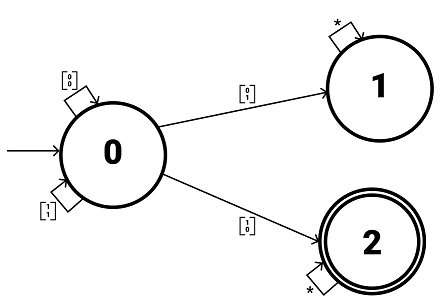
\includegraphics{DFA24}
\end{center}

به ازای دریافت حالت
$\binom{1}{0}$
می‌دانیم عدد بالایی بزرگتر خواهد بود و برای
$\binom{0}{1}$
عدد پایینی. در مابقی حالات در وضعیت خود می‌مانیم.

برای زبان
$L_2$
می‌دانیم هر رشته‌ای که در بالا تکرار شود معکوس همان رشته می‌بایست در پایین تکرار شود. بنابراین یک حالت آن می‌تواند به صورت زیر باشد.
$$\mqty[1^p & 0^p \\ 0^p & 1^p] = x y z$$
که در آن
$|x y| \leq p$
و
$|y| > 0$
خواهند بود. پس می‌توان گفت
$y$
به صورت
$\binom{1^k}{0^k},\, 0 < k < p$
خواهد بود.

حالا در رشته‌ی می‌بینیم
$x y^2 z$
که به
$\mqty[1^{p + k} & 0^{p + k} \\ 0^p & 1^p]$
برمی‌خوریم، بنابراین این زبان را نمی‌توان با
DFA
خاصی توصیف کرد و یک زبان نامنظم است.

\subsection*{۲.۳}

با استفاده از لم پمپاژ اثبات می‌کنیم که این زبان منظم نیست. طبق لم پمپاژ عدد p را پیدا می‌کنیم در ابتدا.

یک رشته‌ی شامل p تا پرانتز باز و p تا پرانتز بسته در نظر بگیرید.

با توجه به این‌که

$$s = xyz,\,|x y| < p, |y| > 0$$

پس داریم که y شامل تعدادی پرانتز باز است فقط.

حالا با توجه به لم پمپاژ به ازای هر i، یک عضو زبان گفته می‌شود به هر 
$x y^i z$

اما در این‌جا با قرار دادن i به مقدار ۲، تعداد پرانتزهای باز از بسته بیشتر می‌شود و رشته خوش‌پرانتز نیست. 

در نتیجه لم پمپاژ صدق نمی‌کند و زبان منظم نیست.

\subsection*{۳.۳}

می‌توان با استفاده از زبان
$L_1 = \{a^i b^i\,|\,i > 0\}$
نشان داد که زبان
$L_2$
نامنظم است. برای زبان
$L_2$
زبانی را تعریف می‌کنیم که اشتراکش با آن برابر زبان
$L_1$
شود. برای تعریف چنین زبانی می‌توانیم یک زبان که با ۱ شروع می‌شود تعریف کنیم به طوری که حتما ۱ یا ۰ داشته باشد و به تعداد دلخواه تکرار شود، یعنی داریم.
$$L_4 = \{11^{*} 00^{*}\} \implies L_2 \cap L_4 = L_1$$
می‌دانیم که زبان
$L_4$
منظم است چون می‌توان یک
DFA
برای آن طراحی کرد که از دارای سه استیت بوده و با ورود ۱ از استیت شروع به استیت شماره یک می‌رود. در استیت شماره یک با دریافت ورودی صفر به استیت شماره دو و با گرفتن ورودی یک در خود بماند. برای استیت شماره دو هم فقط در حالتی که ورودی، صفر باشد، در خود می‌ماند و حالت
$accept$
خواهد بود.
حالا چون اشتراک زبان
$L_2$
با زبان دیگری منظم نبود، پس این زبان نامنظم است.

برای بخش دوم این سوال، فرض می‌کنیم 
$L_5$
زبانی شامل تمام رشته‌های شامل دقیقا یک عدد ۰ است. این زبان منظم است و عبارت منظم آن به شکل 
$$
(1 \cup 2)^* 0(1 \cup 2)^*
$$
است.
حالا اگر 
$L_3$
منظم باشد، با توجه به خواص بستاری زبان 
$L_3 \cap L'$
هم منظم است که این زبان معادل زبان
$\{ 01^y2^y | y \geq 0 \}$

حال چون یک DFA برای این زبان وجود دارد که 
$0 \notin \{ 1, 2\}$
پس 	
quotient left
این زبان نسبت به 
$\{ 0 \}$
می‌شود:
$\{ 1^y2^y | y \geq 0 \}$
که زبان نامنظمی است و تناقض داریم و بدست می‌آید که 
$L_3$
نامنظم است.